\section{Technique}


This scheme is beneficial in cases with a high ratio of communication to computation and a non-negligible overhead associated with sending messages.


\begin{figure}
  \centering
  \documentclass[tikz]{standalone}

\begin{document}
  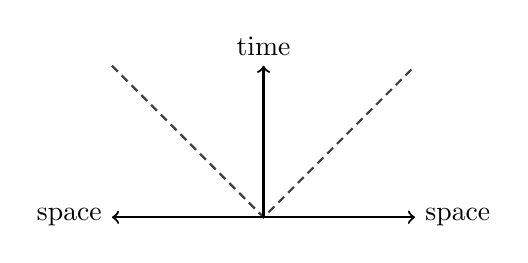
\begin{tikzpicture}[scale=0.35]
    \draw[thick, darkgray, densely dashed] (0, 6) -- (5.5, 0.5) -- (11, 6);
    \draw[thick,->] (5.5,0.5) -- (5.5, 6) node (yaxis) [above] {time}; 
    \draw[thick, <->] (0,0.5) node [left] {space} -- (11,0.5) node (xaxis) [right] {space};
  \end{tikzpicture}
\end{document}

  \caption{Space-Time Diagram}
  \label{fig:lightcone}
\end{figure}


\begin{figure}
  \centering
  \documentclass[tikz]{standalone}

% https://www.sharelatex.com/blog/2013/08/27/tikz-series-pt1.html
\usepackage{tikz}
\begin{document}
\definecolor{printred}{RGB}{215,25,28}
\definecolor{printblue}{RGB}{43,131,186}
\begin{tikzpicture}[scale=0.35]

  % Drawing parameters
  \pgfmathsetmacro{\maxy}{5}%
  \pgfmathsetmacro{\neighbourinnerwidth}{3}%
  \pgfmathsetmacro{\centerinnerwidth}{5}%
  \pgfmathsetmacro{\gapwidth}{2}%
  \pgfmathsetmacro{\borderwidth}{1}%
  \pgfmathsetmacro{\arrowdisplacement}{1.5}

  % Intermezzo values
  \pgfmathsetmacro{\centerxanchor}{\neighbourinnerwidth+\borderwidth+\gapwidth}
  \pgfmathsetmacro{\rightxanchor}{\centerxanchor+\borderwidth*2+\centerinnerwidth+\gapwidth}

  %% Here Be Dragons!
  % Ghost Columns
  \fill[lightgray](\neighbourinnerwidth,0) rectangle (\neighbourinnerwidth+\borderwidth,\maxy);
  \fill[lightgray] (\centerxanchor,0) rectangle (\centerxanchor+\borderwidth,\maxy);
  \fill[lightgray] (\centerxanchor+\borderwidth+\centerinnerwidth,0) rectangle (\centerxanchor+\borderwidth*2+\centerinnerwidth,\maxy);
  \fill[lightgray](\rightxanchor,0) rectangle (\rightxanchor+\borderwidth,\maxy);

  % Grids
  \draw[step=1, gray, very thin] (0,0) grid (\neighbourinnerwidth+\borderwidth,\maxy);
  \draw[step=1, gray, very thin] (\centerxanchor,0) grid (\centerxanchor+\centerinnerwidth+2*\borderwidth,\maxy);
  \draw[step=1, gray, very thin] (\rightxanchor,0) grid (\rightxanchor+\neighbourinnerwidth+\borderwidth,\maxy);

  % Left-To-Right transmission (->)
  \draw[printred, densely dashed, thick](\neighbourinnerwidth-\borderwidth,0) rectangle (\neighbourinnerwidth,\maxy);
  \draw[->] (\neighbourinnerwidth-\borderwidth/2,\maxy-\arrowdisplacement) -- (\centerxanchor+.5*\borderwidth,\maxy-\arrowdisplacement);
  \draw[printred, densely dashed, thick](\centerxanchor+\centerinnerwidth,0) rectangle (\centerxanchor+\borderwidth+\centerinnerwidth,\maxy);
  \draw[->] (\centerxanchor+\centerinnerwidth+.5*\borderwidth,\maxy-\arrowdisplacement) -- (\rightxanchor+.5*\borderwidth,\maxy-\arrowdisplacement);

  % Right-To-Left transmission (<-)
  \draw[printblue, densely dashed, thick] (\centerxanchor+\borderwidth,0) rectangle (\centerxanchor+2*\borderwidth,\maxy);
  \draw[->] (\centerxanchor+1.5*\borderwidth, \arrowdisplacement) -- (\neighbourinnerwidth+.5*\borderwidth, \arrowdisplacement);
  \draw[printblue, densely dashed, thick] (\rightxanchor+\borderwidth,0) rectangle (\rightxanchor+2*\borderwidth,\maxy);
  \draw[->] (\rightxanchor+1.5*\borderwidth, \arrowdisplacement) -- (\centerxanchor+\centerinnerwidth+1.5*\borderwidth, \arrowdisplacement);

\end{tikzpicture}
\end{document}

  \caption{Conventional 1D Boundary Exchange}
  \label{fig:exch1d}
\end{figure}

\begin{figure}
  \centering
  \documentclass[tikz]{standalone}

% https://www.sharelatex.com/blog/2013/08/27/tikz-series-pt1.html
\usepackage{tikz}
\usetikzlibrary{patterns}
\begin{document}
\definecolor{printred}{RGB}{215,25,28}
\begin{tikzpicture}[scale=0.35]

  % Drawing parameters
  \pgfmathsetmacro{\maxy}{5}%
  \pgfmathsetmacro{\neighbourinnerwidth}{3}%
  \pgfmathsetmacro{\centerinnerwidth}{5}%
  \pgfmathsetmacro{\gapwidth}{2}%
  \pgfmathsetmacro{\borderwidth}{1}%
  
  % Intermezzo values
  \pgfmathsetmacro{\centerxanchor}{\neighbourinnerwidth+\borderwidth+\gapwidth}
  \pgfmathsetmacro{\rightxanchor}{\centerxanchor+\borderwidth*2+\centerinnerwidth+\gapwidth}


  %% Here Be Dragons!

  % Discarded Columns
  \draw[pattern color=lightgray, pattern=north west lines, very thin](\neighbourinnerwidth,0) rectangle (\neighbourinnerwidth+\borderwidth,\maxy);
  \draw[pattern color=lightgray, pattern=north west lines, very thin](\centerxanchor+\borderwidth+\centerinnerwidth,0) rectangle (\centerxanchor+\borderwidth*2+\centerinnerwidth,\maxy);
 
  % Ghost Columns
  \fill[lightgray](\neighbourinnerwidth-\borderwidth,0) rectangle (\neighbourinnerwidth,\maxy);
  \fill[lightgray] (\centerxanchor-\borderwidth,0) rectangle (\centerxanchor,\maxy);
  \fill[lightgray] (\centerxanchor+\centerinnerwidth,0) rectangle (\centerxanchor+\borderwidth+\centerinnerwidth,\maxy);
  \fill[lightgray](\rightxanchor-\borderwidth,0) rectangle (\rightxanchor,\maxy);

  % Grids
  \draw[step=1, gray, very thin] (0,0) grid (\neighbourinnerwidth,\maxy);
  \draw[step=1, gray, very thin] (\centerxanchor-\borderwidth,0) grid (\centerxanchor+\centerinnerwidth+\borderwidth,\maxy);
  \draw[step=1, gray, very thin] (\rightxanchor-\borderwidth,0) grid (\rightxanchor+\neighbourinnerwidth+\borderwidth,\maxy);

  % Left-To-Right transmission (->)
  \draw[printred, densely dashed, thick](\neighbourinnerwidth-2*\borderwidth,0) rectangle (\neighbourinnerwidth,\maxy);
  \draw[->] (\neighbourinnerwidth-\borderwidth,.5*\maxy) -- (\centerxanchor,.5*\maxy);
  \draw[printred, densely dotted, thick] (\centerxanchor-\borderwidth,0) rectangle (\centerxanchor+\borderwidth,\maxy);
  \draw[printred, densely dashed, thick](\centerxanchor+\centerinnerwidth-\borderwidth,0) rectangle (\centerxanchor+\borderwidth+\centerinnerwidth,\maxy);
  \draw[->] (\centerxanchor+\centerinnerwidth,.5*\maxy) -- (\rightxanchor,.5*\maxy);
  \draw[printred, densely dotted, thick] (\rightxanchor-\borderwidth,0) rectangle (\rightxanchor+\borderwidth,\maxy);

\end{tikzpicture}
\end{document}

  \caption{Cascade 1D Boundary Exchange}
  \label{fig:casc1d}
\end{figure}

\subsection{Streaming Communications}
\begin{figure}
  \centering
  \documentclass[tikz]{standalone}

\begin{document}
  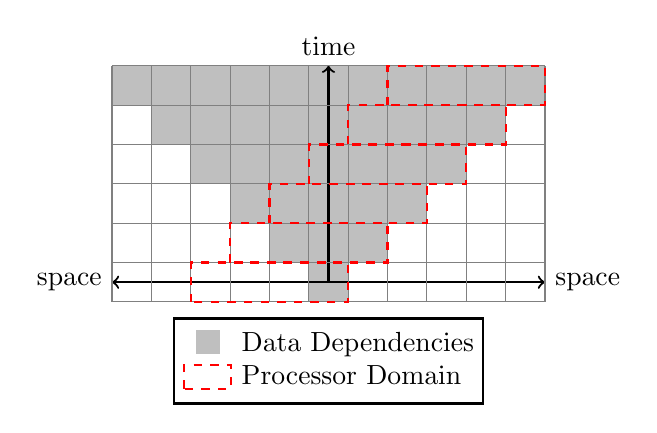
\begin{tikzpicture}[scale=0.5]
    \fill[lightgray] (0,5) rectangle (11, 6);
    \fill[lightgray] (1,4) rectangle (10, 5);
    \fill[lightgray] (2,3) rectangle (9, 4);
    \fill[lightgray] (3,2) rectangle (8, 3);
    \fill[lightgray] (4,1) rectangle (7, 2);
    \fill[lightgray] (5,0) rectangle (6, 1);
    \draw[thick,->] (5.5,0.5) -- (5.5, 6) node (yaxis) [above] {time}; 
    \draw[thick, <->] (0,0.5) node [left] {space} -- (11,0.5) node (xaxis) [right] {space};
    \draw[gray, step=1] (0,0) grid (11,6);
    \foreach \ts in {0,...,5} {
      \draw[thick, dashed, red] (\ts+2,\ts) rectangle (\ts+6,\ts+1);
    }

    \node[draw=black,thick] at (5.5, -1.5) {%
      \begin{tabular}{@{}c@{ }l@{}}
        \raisebox{-1pt}{\tikz{\fill[lightgray] (0,0) rectangle (3mm,3mm);}} & Data Dependencies\\
        \raisebox{-2pt}{\tikz{\draw[thick, dashed, red] (0,0) rectangle (6mm,3mm);}} & Processor Domain\\
      \end{tabular}
    };
  \end{tikzpicture}
\end{document}

  \caption{Simulation Dependencies}
  \label{fig:simcone}
\end{figure}

\begin{figure}
  \booltrue{commstl}
  \booltrue{commsbl}
  \centering
  \documentclass[tikz]{standalone}
\usepackage{etoolbox} % for toggles

\newbool{commstr}
\newbool{commstl}
\newbool{commsbr}
\newbool{commsbl}

\booltrue{commstr}
\booltrue{commstl}
\booltrue{commsbr}
\booltrue{commsbl}

\begin{document}
\tikzstyle{proc} = [circle, draw=black, fill=lightgray]

\begin{tikzpicture}[]
  \matrix[row sep=0.75cm, column sep=1.5cm] {
    \node (A3) [proc] {}; &  \node (B3) [proc] {}; &  \node (C3) [proc] {}; \\
    \node (A2) [proc] {}; &  \node (B2) [proc] {}; &  \node (C2) [proc] {}; \\
    \node (A1) [proc] {}; &  \node (B1) [proc] {}; &  \node (C1) [proc] {}; \\
  };
 
  % Vertical dashed continuity lines
  \path[->]
    (A1) edge[thick, dashed] (A2) 
    (B1) edge[thick, dashed] (B2)
    (C1) edge[thick, dashed] (C2)
    (A2) edge[thick, dashed] (A3) 
    (B2) edge[thick, dashed] (B3)
    (C2) edge[thick, dashed] (C3)
  ;
 
  % Bottom level --> arrows
  \ifbool{commsbr}{
    \path[->]
      (A1) edge[thick] (B2)
      (B1) edge[thick] (C2)
    ;
  }{}
  % Bottom level <-- arrows
  \ifbool{commsbl}{
    \path[->]
      (B1) edge[thick] (A2)
      (C1) edge[thick] (B2)
    ;
  }{}
  % Top level --> arrows
  \ifbool{commstr}{
    \path[->]
      (A2) edge[thick] (B3)
      (B2) edge[thick] (C3)
    ;
  }{}
  % Top level <-- arrows
  \ifbool{commstl}{
    \path[->]
      (B2) edge[thick] (A3)
      (C2) edge[thick] (B3)
    ;
  }{}
  \end{tikzpicture}
\end{document}

  \caption{Streaming Communications Pattern}
  \label{fig:streamingcomms}
\end{figure}

\begin{figure}
  \centering
  \documentclass[tikz]{standalone}
\usetikzlibrary{patterns}
\begin{document}
  \tikzset{>=latex} % Change default arrowhead to filled triangle
  \def\stencil[#1, #2]{% x, y
    \draw[very thick, red] (#1+1, #2) rectangle (#1+2, #2-3);
    \draw[very thick, red] (#1, #2-1) rectangle (#1+3, #2-2);
  }

  \begin{tikzpicture}[scale=0.5]

    \draw[gray, step=1] (0,0) grid (3,8);
    \node at(0.5, 8.5) {\emph{0}}; \node at(1.5, 8.5) {\emph{1}}; \node at(2.5, 8.5) {\emph{2}};
    \draw[pattern color=lightgray, pattern=north west lines, very thin](0, 0) rectangle (1, 3);
    \draw[pattern color=lightgray, pattern=north west lines, very thin](1, 0) rectangle (2, 8);
    \draw[pattern color=lightgray, pattern=north west lines, very thin](2, 2) rectangle (3, 8);
    \node at(1.5, -0.75) {\emph{t}};
    \stencil[0, 4]
    
    \draw[gray, step=1] (5,0) grid (8,8);
    \node at(6.5, 9.5) {\emph{columns}};
    \node at(5.5, 8.5) {\emph{1}}; \node at(6.5, 8.5) {\emph{2}}; \node at(7.5, 8.5) {\emph{3}};
    \draw[pattern color=lightgray, pattern=north west lines, very thin](5, 0) rectangle (6, 4);
    \draw[pattern color=lightgray, pattern=north west lines, very thin](6, 0) rectangle (7, 8);
    \draw[pattern color=lightgray, pattern=north west lines, very thin](7, 3) rectangle (8, 8);
    \node at(6.5, -0.75) {\emph{t+1}};
    \node at(6.5, -1.75) {\emph{timesteps}};
    \stencil[5, 5]

    \draw[gray, step=1] (10,0) grid (13,8);
    \node at(10.5, 8.5) {\emph{2}}; \node at(11.5, 8.5) {\emph{3}}; \node at(12.5, 8.5) {\emph{4}};
    \draw[pattern color=lightgray, pattern=north west lines, very thin](10, 0) rectangle (11, 5);
    \draw[pattern color=lightgray, pattern=north west lines, very thin](11, 0) rectangle (12, 8);
    \draw[pattern color=lightgray, pattern=north west lines, very thin](12, 4) rectangle (13, 8);
    \node at(11.5, -0.75) {\emph{t+2}};
    \stencil[10, 6]

    % Communications arrows
    \path[->]
    (1.5, 2.5) edge[bend right] (7.5, 2.5)
    (6.5, 3.5) edge[bend right] (12.5, 3.5);

  \end{tikzpicture}
\end{document}

  \caption{SSA Architecture}
  \label{fig:ssa_concept}
\end{figure}


\begin{table}
  \scriptsize
  \centering
  \caption{Stencil Code Architecture Comparrison}
  \label{tab:comparrison}
  \begin{tabular}{@{}cccc@{}} \toprule
Metric & SAA & SCMA & Mine \\
\midrule
  Stencils/Message & 1 & 2 & 3 \\
  Stencils/Bandwidth & 1 & 2 & 3 \\
  Maximum parallelism & 1 & 2 & 3 \\
\bottomrule
\end{tabular}

\end{table}

\subsection{Alternating Communications}

Requires half-duplex communications links between processing elements.
\begin{figure}
  \booltrue{commstr}
  \booltrue{commsbl}
  \centering
  \documentclass[tikz]{standalone}
\usepackage{etoolbox} % for toggles

\newbool{commstr}
\newbool{commstl}
\newbool{commsbr}
\newbool{commsbl}

\booltrue{commstr}
\booltrue{commstl}
\booltrue{commsbr}
\booltrue{commsbl}

\begin{document}
\tikzstyle{proc} = [circle, draw=black, fill=lightgray]

\begin{tikzpicture}[]
  \matrix[row sep=0.75cm, column sep=1.5cm] {
    \node (A3) [proc] {}; &  \node (B3) [proc] {}; &  \node (C3) [proc] {}; \\
    \node (A2) [proc] {}; &  \node (B2) [proc] {}; &  \node (C2) [proc] {}; \\
    \node (A1) [proc] {}; &  \node (B1) [proc] {}; &  \node (C1) [proc] {}; \\
  };
 
  % Vertical dashed continuity lines
  \path[->]
    (A1) edge[thick, dashed] (A2) 
    (B1) edge[thick, dashed] (B2)
    (C1) edge[thick, dashed] (C2)
    (A2) edge[thick, dashed] (A3) 
    (B2) edge[thick, dashed] (B3)
    (C2) edge[thick, dashed] (C3)
  ;
 
  % Bottom level --> arrows
  \ifbool{commsbr}{
    \path[->]
      (A1) edge[thick] (B2)
      (B1) edge[thick] (C2)
    ;
  }{}
  % Bottom level <-- arrows
  \ifbool{commsbl}{
    \path[->]
      (B1) edge[thick] (A2)
      (C1) edge[thick] (B2)
    ;
  }{}
  % Top level --> arrows
  \ifbool{commstr}{
    \path[->]
      (A2) edge[thick] (B3)
      (B2) edge[thick] (C3)
    ;
  }{}
  % Top level <-- arrows
  \ifbool{commstl}{
    \path[->]
      (B2) edge[thick] (A3)
      (C2) edge[thick] (B3)
    ;
  }{}
  \end{tikzpicture}
\end{document}

  \caption{Alternating Communications Pattern}
  \label{fig:alternatingcomms}
\end{figure}


\subsection{Hybrid Schemes}

